\documentclass[11pt,a4paper]{ctexart}

\usepackage{amsmath,amssymb,bm}
\usepackage{geometry}
\usepackage{enumitem}
\usepackage{fancyhdr}
\usepackage{lastpage}
\usepackage{xcolor}
\usepackage{tcolorbox}
\usepackage{tikz}
\usepackage{titlesec}
\usepackage{microtype}
\usepackage{graphicx}
\usetikzlibrary{arrows.meta,calc}

\geometry{left=2.15cm,right=2.15cm,top=2.0cm,bottom=2.0cm}
\setlength{\parindent}{2em}
\setlength{\parskip}{0.25em}
\linespread{1.12}
\graphicspath{{figures/}}

\definecolor{mainblue}{RGB}{39,91,150}
\definecolor{lightblue}{RGB}{232,241,252}
\definecolor{darkgray}{RGB}{65,65,65}
\definecolor{lightgray}{RGB}{245,246,248}

\titleformat{\section}{\large\bfseries\color{mainblue}}{}{0em}{}[\titlerule]
\titleformat{\subsection}{\normalsize\bfseries\color{darkgray}}{}{0em}{}
\titlespacing*{\section}{0pt}{0.9em}{0.45em}
\titlespacing*{\subsection}{0pt}{0.65em}{0.25em}

\setlist[enumerate]{leftmargin=2.2em,itemsep=0.25em,topsep=0.25em}
\setlist[itemize]{leftmargin=2.0em,itemsep=0.2em,topsep=0.2em}

\pagestyle{fancy}
\fancyhf{}
\lhead{\small 格物助航｜每日一练}
\rhead{\small 2026.6.10}
\cfoot{\small 第 \thepage\ 页 / 共 \pageref{LastPage} 页}
\renewcommand{\headrulewidth}{0.4pt}

\newtcolorbox{problemBox}{
  colback=lightblue,
  colframe=mainblue,
  arc=2mm,
  boxrule=0.7pt,
  left=1.0em,
  right=1.0em,
  top=0.8em,
  bottom=0.8em,
  before skip=0.6em,
  after skip=0.8em
}

\newtcolorbox{tipBox}{
  colback=lightgray,
  colframe=darkgray,
  arc=1.5mm,
  boxrule=0.5pt,
  left=0.9em,
  right=0.9em,
  top=0.6em,
  bottom=0.6em,
  before skip=0.5em,
  after skip=0.5em
}

\newcommand{\dd}{\mathrm{d}}

\begin{document}

\begin{center}
  {\Large\bfseries\color{mainblue} 格物助航｜每日一练}\par
  \vspace{0.25em}
  {\large 力学第五章：角动量定理与角动量守恒定律}\par
  \vspace{0.35em}
  {\small 2026年6月10日}\par
  \vspace{0.35em}
  {\small 编写：罗琦皓}
\end{center}

\vspace{-0.3em}

\begin{problemBox}
\noindent\textbf{题目}\quad
水平光滑桌面上有一质量为 $m$ 的小球，系在轻绳一端，轻绳穿过桌面上的小孔 $O$。初始时小球以角速度 $\omega_0$ 在半径为 $R$ 的圆周上绕 $O$ 匀速运动。现缓慢向下拉绳，使小球始终可近似看作绕 $O$ 作圆周运动，半径从 $R$ 缩小到 $R/2$。忽略绳的质量和一切摩擦。求：
\begin{enumerate}
  \item 拉绳过程中小球对 $O$ 点的角动量是否守恒？说明理由；
  \item 半径为 $r$ 时小球的速率 $v(r)$ 与角速度 $\omega(r)$，并求最终的 $v_f$、$\omega_f$；
  \item 拉力对小球所做的功；
  \item 小球的机械能是否守恒？为什么？
\end{enumerate}
\end{problemBox}

\begin{center}
  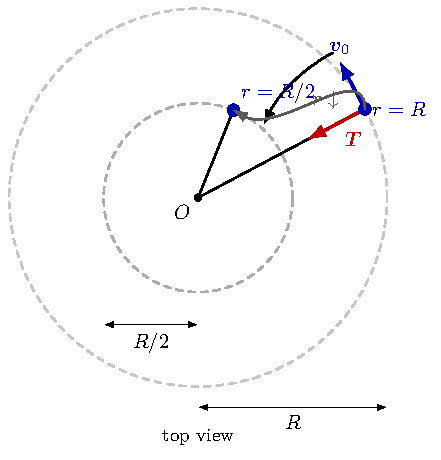
\includegraphics[width=0.48\textwidth]{pull_string.pdf}\par
  {\small 图示为小球在水平桌面上的俯视图，绳的拉力始终沿径向指向 $O$。}
\end{center}

\section*{详细解法}

\subsection*{一、判断守恒量}

取过小孔 O 的竖直轴为参考轴。小球在水平面内运动，重力和支持力均不产生关于该竖直轴的力矩；绳的拉力沿径向，作用线通过 O，关于该轴的力矩也为零。因此关于 O 轴的角动量守恒。若从矢量角动量角度看，重力与支持力的合力为零，拉力对 O 点的力矩为零，所以合外力矩为零：
\[
  \bm M_O=\bm r\times \bm T=\bm 0 .
\]
由角动量定理
\[
  \frac{\dd \bm L_O}{\dd t}=\bm M_O,
\]
可知小球对 $O$ 点的角动量守恒。
初始角动量大小为
\[
  L=mR^2\omega_0.
\]

\subsection*{二、求半径为 $r$ 时的速率与角速度}

半径为 $r$ 时，若小球仍近似作圆周运动，则
\[
  L=mrv=m r^2\omega .
\]
由角动量守恒得
\[
  mrv=mR^2\omega_0,
  \qquad
  mr^2\omega=mR^2\omega_0.
\]
因此
\[
  \boxed{v(r)=\frac{R^2\omega_0}{r}},
  \qquad
  \boxed{\omega(r)=\frac{R^2\omega_0}{r^2}}.
\]
当 $r=R/2$ 时，
\[
  \boxed{v_f=2R\omega_0},
  \qquad
  \boxed{\omega_f=4\omega_0}.
\]

\subsection*{三、求拉力做功}

初态动能为
\[
  K_i=\frac12 m(R\omega_0)^2
      =\frac12 mR^2\omega_0^2 .
\]
末态动能为
\[
  K_f=\frac12 m(2R\omega_0)^2
      =2mR^2\omega_0^2 .
\]
重力和支持力不做功，拉力是唯一改变小球动能的力，所以由动能定理
\[
  A_T=K_f-K_i
      =\boxed{\frac32 mR^2\omega_0^2}.
\]
也可以从拉力积分验证。半径为 $r$ 时向心力由绳的拉力提供：
\[
  T(r)=m\frac{v^2}{r}
      =m\frac{R^4\omega_0^2}{r^3}.
\]
拉绳时位移沿径向向内，$\dd r<0$，故
\[
\begin{aligned}
  A_T
  &=\int_R^{R/2}T(r)(-\dd r)  \\
  &=\int_R^{R/2}-mR^4\omega_0^2r^{-3}\dd r
   =\frac32 mR^2\omega_0^2 .
\end{aligned}
\]

\subsection*{四、判断机械能是否守恒}

小球的动能从
\[
  \frac12 mR^2\omega_0^2
\]
增加到
\[
  2mR^2\omega_0^2 .
\]
因此小球的机械能不守恒。原因是：外力矩为零只保证角动量守恒；拉力虽然对 $O$ 点无力矩，但在半径缩短的过程中沿小球的径向位移做正功，所以小球动能增加。

\section*{技巧与知识点}

\begin{tipBox}
\begin{enumerate}
  \item \textbf{角动量守恒条件：}判断的是对同一点的合外力矩是否为零，即 $\bm M_O=\bm 0$，而不是合外力是否为零。
  \item \textbf{径向力可做功：}拉力过 $O$，所以力矩为零；但半径变小时，小球有径向位移，所以拉力可以做功。
  \item \textbf{圆周运动的角动量：}对圆心有 $L=mrv=mr^2\omega$。半径变小时，$v$ 与 $\omega$ 都会增大。
  \item \textbf{常见易错点：}角动量守恒并不推出机械能守恒。是否守恒要分别看外力矩和外力做功。
\end{enumerate}
\end{tipBox}

\section*{复习建议}

第五章复习时建议把题目先分成两步：第一步只判断力矩，确定是否能用角动量守恒；第二步再判断做功，确定机械能或动能如何变化。遇到有心力、拉绳缩短半径、行星掠面速度这类题，都应优先写出
\[
  \bm L=\bm r\times m\bm v,
  \qquad
  \frac{\dd\bm L}{\dd t}=\bm M.
\]
如果题目还问速度、角速度或做功，再把 $L=mrv=mr^2\omega$ 与动能定理结合使用。

\end{document}
